\subsection{Supplementary Services}

As the other branches of the prototyping where happening, the need for additional services and infrastructure arose to 
support the development of the prototype as well as to increase the general usability of the prototype. 
This section will especially describe the services which help to make this prototype a more complete solution.


\begin{figure}[htb]
    \centering
    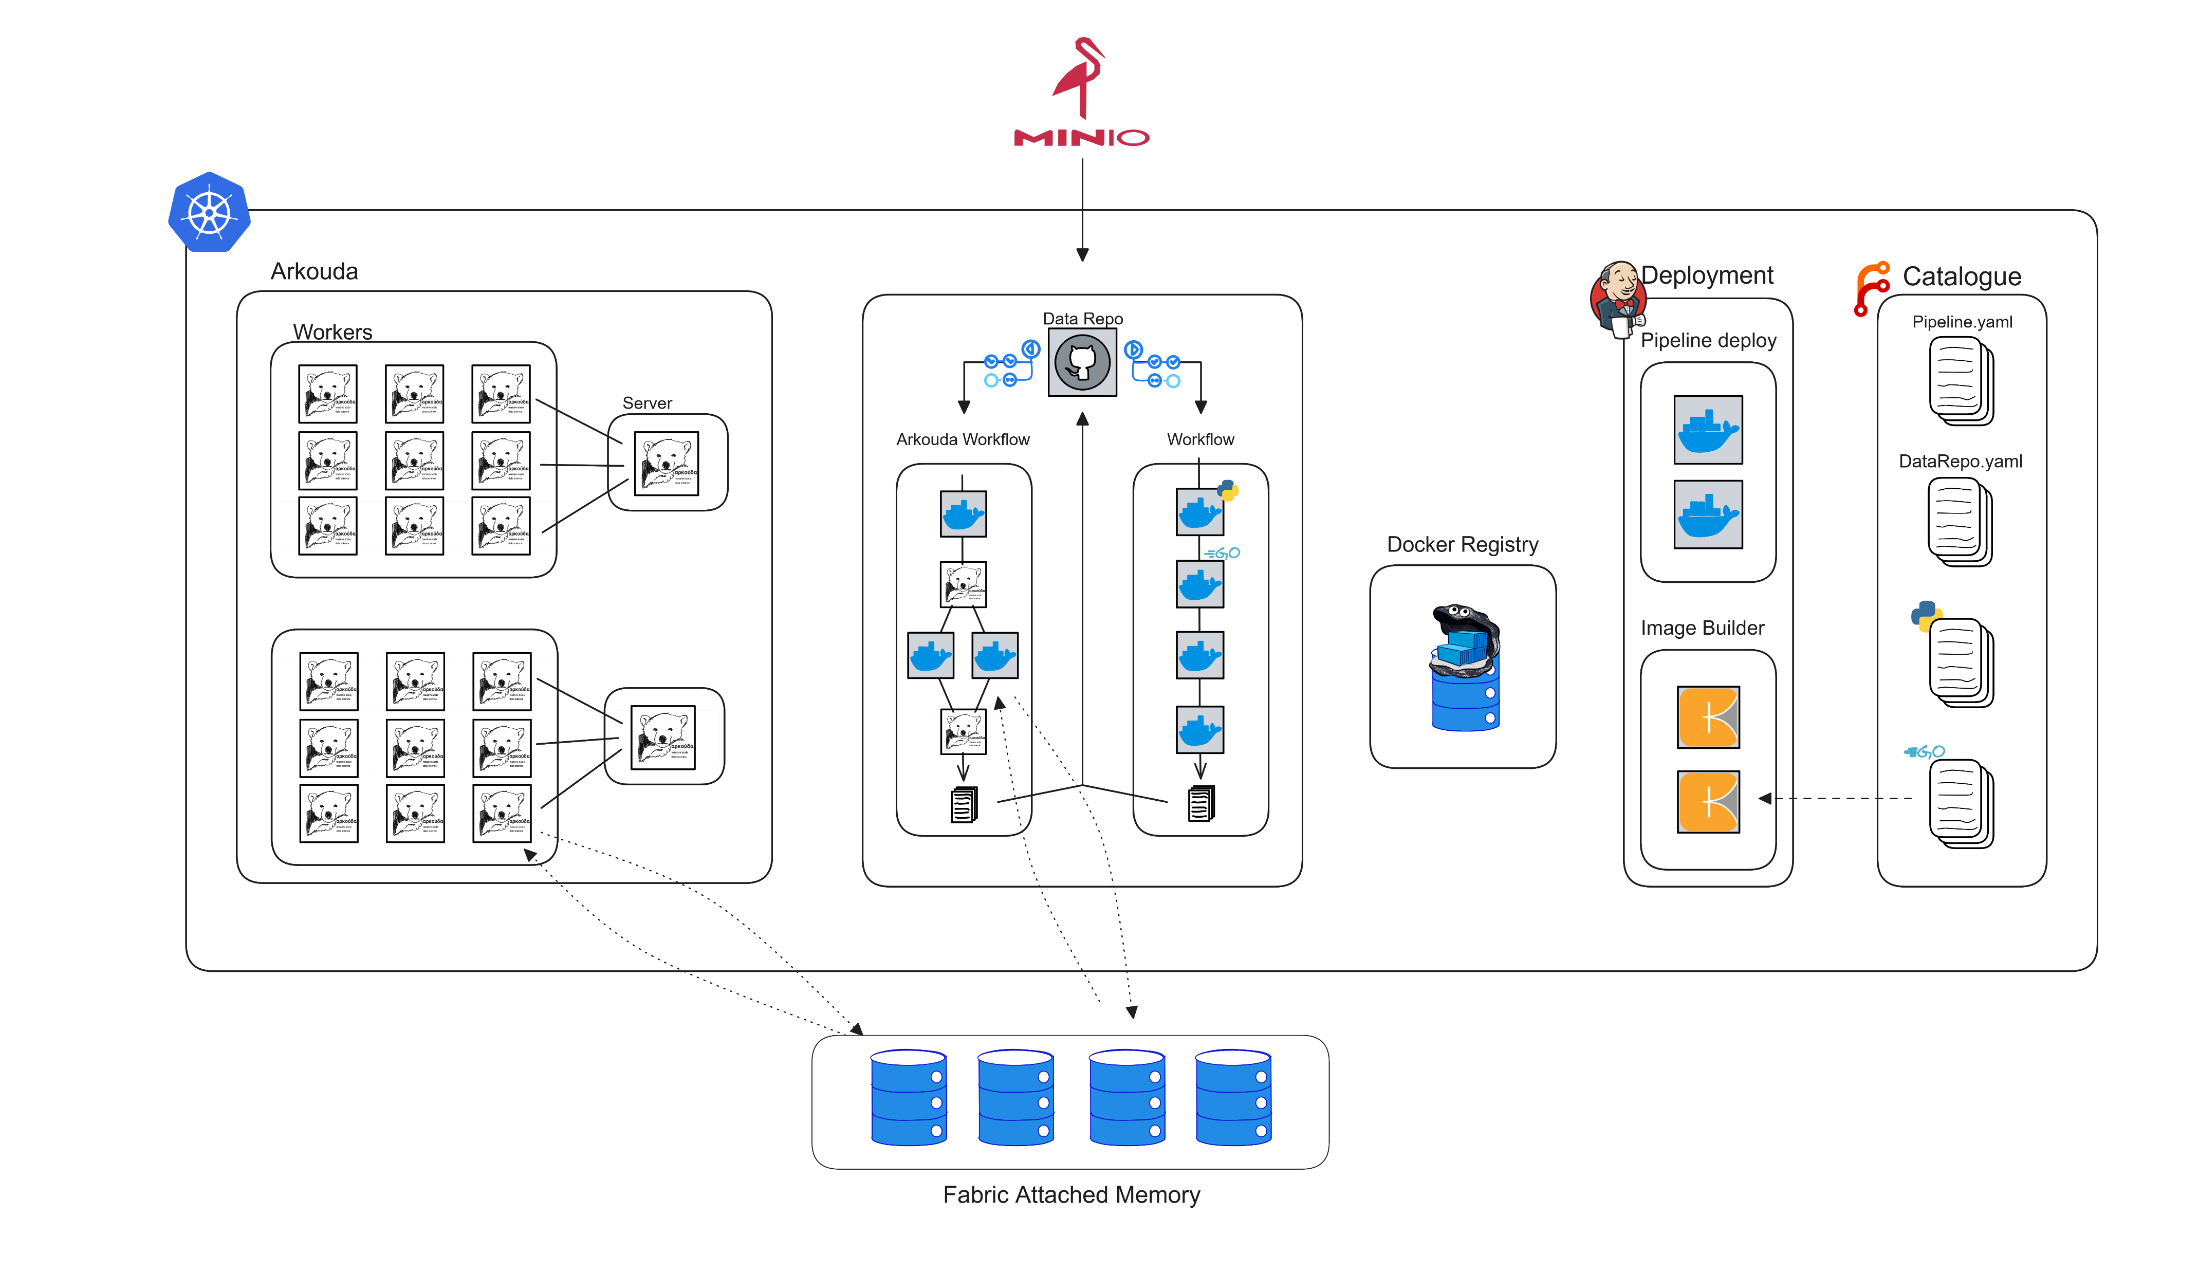
\includegraphics[width=17cm]{graphics/pachykouda_complete.png}
    \caption[Pachyderm High-Level Architecture]{Pachyderm High-Level Architecture}
    \label{abb:pachyderm_complete}
\end{figure}

\subsubsection{Docker Registry}

One thing that was quite apparent from the get go, was the need for a central docker registry.
As Pachyderm does not manage the docker images itself, but relies on the user to provide them somehow externally.

During the first iterations when the development was being done on Minikube as described in \ref{minikube}, the internal Registry 
of the node was enough.
But as soon as we moved over to the Heydar system keeping the Hosts internal registries in sync was of course not feasible,
Therefore we added a private docker registry to the cluster \footcite{kumarHowSetupPrivate2020}.
The deployment config is based on the official docker registry helm chart\footcite{Dockerregistry10Phntom} and can be found at \ref{appendix:docker_registry_config}.

\subsubsection{Frogejo Catalogue}

As this should be the \ac{POC} of an end user tool, we should also look into usability features and based on previous experience of the team,
the need for a catalogue of previously developed pipelines and processing code was identified.
The idea was to create something similar to the Clasp catalogue\footcite{sayersCLoudApplicationServices2015} but for the Pachyderm ecosystem.
Meaning that users can share, search and deploy workflows from a central catalog, without having to worry about the underlying infrastructure.

Having \ac{HPC} software in a completely contained and version system directly addresses many of the original problem statements,
described in \ref{ProblemStatement}, especially the problem of reproducibility, environment management and the lack of portability.

To start of we, installed a simple github-like interface for the catalogue, called Frogejo\footcite{forgejoForgejo} which is a fork of the \ac{FOSS} project Gitea\footcite{GiteaGitCup2023},
being maintained by the \ac{NPO} Codeberg e.V.\footcite{codebergCodebergOrg}.
The installation was done using their official helm chart\footcite{Forgejo13Forgejo} and can be found at \ref{appendix:frogejo_config}.

\subsubsection{Jenkins CI/CD Pipeline}

Now that we have a place to hold and version the code files and a place to hold the resulting docker images, we need a way to build and deploy them automatically.
For that purpose an installation of Jenkins was added to the Cluster. Jenkins is a \ac{FOSS} \ac{CI/CD} tool, which is widely used in industry \footcite{JenkinsMarketShare}.
It enables us to automatically build and deploy docker images whenever code is pushed to the Frogejo catalogue, as well as automatically deploying pipeline scripts to Pachyderm.

By using this we ensure that the code and the docker images are always in sync and that the user does not have to worry about building and deploying the images manually or interacting with the underlying Cluster.
We also extend the factor of provenance which was so far limited to the data itself, to the containers code and pipeline spec as well, now having total oversight into which input begets what output.

This was achieved in multiple steps as this turned out to be quite an involved process.
First of was of course the general installation of the project into the Cluster based on the image provided by Jenkins \footcite{JenkinsJenkinsJenkinsci}.
And its integration into the Kubernetes cluster, as we want it to be able to spawn its own worker pods within the cluster to handle the building of the containers and pushing of the pipelines, 
the description of how to set up the permissions in the 1, as well as the \ac{CaC} file for the Jenkins installation can be found at \ref{appendix:jenkins_config}.

        